\documentclass[11pt,a4paper]{article}
\usepackage[margin=0.75in]{geometry}
\usepackage{amsmath,amssymb}
\usepackage{tikz}
\usepackage{graphicx}
\usepackage{enumitem}
\usepackage{xcolor}
\usepackage{tcolorbox}
\usepackage{booktabs}

\usetikzlibrary{shapes,arrows,positioning}

\title{\textbf{Feature Selection \& Principal Component Analysis (PCA)\\Viva Examination Guide}}
\author{Comprehensive Conceptual Overview}
\date{\today}

\definecolor{conceptblue}{RGB}{51,102,187}
\definecolor{warningred}{RGB}{204,51,51}

\begin{document}

\maketitle

\section{Definitions and Core Concepts}

\subsection{Feature Selection}
\textbf{Feature Selection} is the process of selecting a subset of relevant features (variables, predictors) from a larger set for use in model construction. It aims to improve model performance, reduce overfitting, decrease training time, and enhance model interpretability.

\textbf{Key Types:}
\begin{itemize}[leftmargin=*]
    \item \textbf{Filter Methods:} Select features based on statistical measures (correlation, chi-square, mutual information) independent of any machine learning algorithm.
    \item \textbf{Wrapper Methods:} Use a predictive model to evaluate feature subsets (forward selection, backward elimination).
    \item \textbf{Embedded Methods:} Feature selection occurs during model training (LASSO, Ridge regression, tree-based feature importance).
\end{itemize}

\subsection{Principal Component Analysis (PCA)}
\textbf{PCA} is a dimensionality reduction technique that transforms original features into a new set of uncorrelated variables called \textbf{principal components}, ordered by the amount of variance they explain. It is a \textit{feature extraction} method (creates new features) rather than feature selection (chooses existing features).

\textbf{Core Principle:} PCA projects high-dimensional data onto lower-dimensional space while preserving maximum variance, identifying directions (principal components) along which data varies most.

\subsection{Covariance}
\textbf{Covariance} measures how two variables change together. It indicates the direction of the linear relationship between variables.

\textbf{Formula:}
\begin{equation}
\text{Cov}(X,Y) = \frac{1}{n-1}\sum_{i=1}^{n}(x_i - \bar{x})(y_i - \bar{y})
\end{equation}

\textbf{Interpretation:}
\begin{itemize}
    \item Positive covariance: Variables increase together
    \item Negative covariance: One increases as the other decreases
    \item Zero covariance: No linear relationship
    \item \textit{Problem:} Scale-dependent, making magnitude difficult to interpret
\end{itemize}

\subsection{Correlation}
\textbf{Correlation} is the normalized version of covariance, measuring the strength and direction of the linear relationship between two variables. The Pearson correlation coefficient ranges from -1 to +1.

\textbf{Formula:}
\begin{equation}
\rho(X,Y) = \frac{\text{Cov}(X,Y)}{\sigma_X \sigma_Y} = \frac{\sum(x_i - \bar{x})(y_i - \bar{y})}{\sqrt{\sum(x_i - \bar{x})^2}\sqrt{\sum(y_i - \bar{y})^2}}
\end{equation}

\textbf{Interpretation:}
\begin{itemize}
    \item $\rho = +1$: Perfect positive linear relationship
    \item $\rho = -1$: Perfect negative linear relationship
    \item $\rho = 0$: No linear relationship
    \item $|\rho| > 0.7$: Strong correlation (threshold may vary by context)
\end{itemize}

\section{Mathematical Foundations of PCA}

\subsection{The PCA Algorithm}
\textbf{Step-by-step mathematical process:}

\begin{enumerate}
    \item \textbf{Standardize the data:} $z = \frac{x - \mu}{\sigma}$ (mean = 0, variance = 1)
    \item \textbf{Compute covariance matrix:} $\Sigma = \frac{1}{n-1}X^TX$ where $X$ is centered data
    \item \textbf{Calculate eigenvectors and eigenvalues:} $\Sigma v = \lambda v$
    \item \textbf{Sort eigenvectors by eigenvalues:} Largest eigenvalue first
    \item \textbf{Select top $k$ eigenvectors:} Form projection matrix $W$
    \item \textbf{Transform data:} $Y = XW$ (project onto new space)
\end{enumerate}

\subsection{Key Mathematical Concepts}

\textbf{Eigenvectors \& Eigenvalues:}
\begin{itemize}
    \item \textbf{Eigenvectors} of the covariance matrix represent the directions (principal components) of maximum variance
    \item \textbf{Eigenvalues} represent the magnitude of variance along each eigenvector
    \item The largest eigenvalue corresponds to the first principal component (PC1)
\end{itemize}

\textbf{Variance Explained:}
\begin{equation}
\text{Variance explained by PC}_i = \frac{\lambda_i}{\sum_{j=1}^{p}\lambda_j} \times 100\%
\end{equation}

\textbf{Cumulative variance} helps determine how many components to retain (typically aim for 80-95\% cumulative variance).

\begin{center}
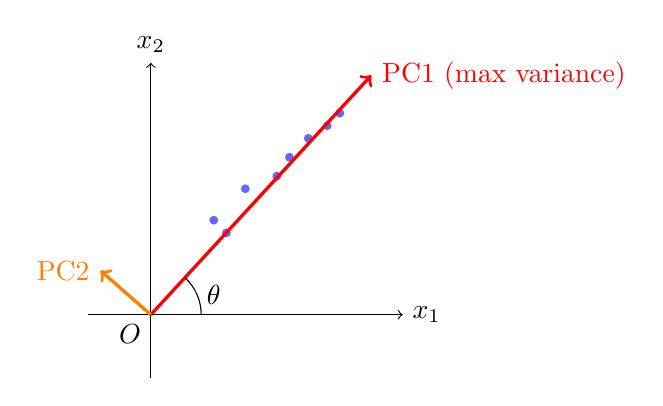
\begin{tikzpicture}[scale=0.8]
% Original axes
\draw[->] (-1,0) -- (4,0) node[right] {$x_1$};
\draw[->] (0,-1) -- (0,4) node[above] {$x_2$};

% Data points
\foreach \x/\y in {1/1.5, 1.5/2, 2/2.2, 2.5/2.8, 3/3.2, 1.2/1.3, 2.2/2.5, 2.8/3}
    \fill[blue!60] (\x,\y) circle (2pt);

% Principal components
\draw[->,very thick,red] (0,0) -- (3.5,3.8) node[right] {PC1 (max variance)};
\draw[->,very thick,orange] (0,0) -- (-0.8,0.7) node[left] {PC2};

% Angle
\draw[dashed] (0,0) -- (3.5,0);
\draw (0.8,0) arc (0:47:0.8) node[midway,right] {$\theta$};

\node[below left] at (0,0) {$O$};
\end{tikzpicture}
\end{center}

\section{Practical Understanding}

\subsection{When to Use Feature Selection}
\begin{itemize}
    \item \textbf{High dimensionality:} Many features relative to samples (curse of dimensionality)
    \item \textbf{Redundant features:} High correlation between features
    \item \textbf{Irrelevant features:} Features with no predictive power
    \item \textbf{Interpretability:} Need simpler, more understandable models
    \item \textbf{Computational constraints:} Reduce training time and memory
\end{itemize}

\subsection{When to Use PCA}
\begin{itemize}
    \item \textbf{Multicollinearity:} Features are highly correlated
    \item \textbf{Visualization:} Project high-dimensional data to 2D/3D
    \item \textbf{Noise reduction:} Remove components with low variance (likely noise)
    \item \textbf{Pre-processing:} Before clustering or regression
    \item \textbf{Data compression:} Store data more efficiently
\end{itemize}

\subsection{PCA Workflow in Practice}
\begin{enumerate}
    \item \textbf{Exploratory Analysis:} Plot feature pairs (F1 vs F2) to identify patterns
    \item \textbf{Check correlation matrix:} Identify redundant features
    \item \textbf{Apply PCA:} Use library function with standardized data
    \item \textbf{Analyze results:} Examine explained variance, scree plot
    \item \textbf{Select components:} Choose $k$ based on cumulative variance
    \item \textbf{Interpret:} Examine loadings to understand component meaning
    \item \textbf{Transform data:} Project original data onto selected PCs
    \item \textbf{Document:} Report variance explained, number of components, justification
\end{enumerate}

\section{Common Viva Questions with Detailed Answers}

\begin{tcolorbox}[colback=conceptblue!5,colframe=conceptblue,title=Q1: Explain the difference between feature selection and feature extraction. Which category does PCA fall into?]
\textbf{Answer:}

\textbf{Feature Selection} chooses a subset of original features without transformation. It maintains interpretability since we keep actual features. Methods include filtering by correlation, wrapper methods, or embedded approaches.

\textbf{Feature Extraction} creates new features by combining or transforming original ones. The new features may be harder to interpret but can capture underlying structure better.

\textbf{PCA is feature extraction} because it creates new features (principal components) as linear combinations of original features. Each PC is: $PC_i = w_{i1}x_1 + w_{i2}x_2 + ... + w_{ip}x_p$

Unlike feature selection (which might keep F1, F3, F5), PCA creates entirely new features (PC1, PC2, PC3) that don't directly correspond to original measurements.
\end{tcolorbox}

\begin{tcolorbox}[colback=conceptblue!5,colframe=conceptblue,title=Q2: Why is standardization important before applying PCA?]
\textbf{Answer:}

Standardization (z-score normalization) is crucial because:

\begin{enumerate}
    \item \textbf{Scale sensitivity:} PCA finds directions of maximum variance. Features with larger scales naturally have larger variance and would dominate the principal components.
    
    \item \textbf{Example:} If F1 is height (150-190 cm) and F2 is weight (0.5-1.2 kg), height's larger numeric range would make PC1 primarily capture height variation, ignoring weight.
    
    \item \textbf{Equal contribution:} Standardization ensures each feature contributes fairly to the analysis based on its variability, not its measurement units.
    
    \item \textbf{Comparability:} Makes covariance matrix more meaningful by converting it to a correlation matrix.
\end{enumerate}

\textbf{Exception:} Don't standardize if features are already on the same scale and the scale difference is meaningful (e.g., all measurements in meters).
\end{tcolorbox}

\begin{tcolorbox}[colback=conceptblue!5,colframe=conceptblue,title=Q3: How do you determine how many principal components to retain?]
\textbf{Answer:}

Multiple criteria can be used:

\begin{enumerate}
    \item \textbf{Cumulative variance threshold:} Retain components explaining 80-95\% of total variance. This is the most common approach.
    
    \item \textbf{Scree plot (Elbow method):} Plot eigenvalues vs component number. Keep components before the "elbow" where curve flattens.
    
    \item \textbf{Kaiser criterion:} Keep components with eigenvalues > 1 (for standardized data). Rationale: components should explain more variance than a single original feature.
    
    \item \textbf{Cross-validation:} If using PCA for prediction, choose $k$ that optimizes model performance on validation data.
    
    \item \textbf{Domain knowledge:} Sometimes interpretability or computational constraints dictate the choice (e.g., 2-3 components for visualization).
\end{enumerate}

\textbf{Trade-off:} More components = more information retained but less dimensionality reduction. Fewer components = more compression but potential information loss.
\end{tcolorbox}

\begin{tcolorbox}[colback=conceptblue!5,colframe=conceptblue,title=Q4: What does the covariance matrix represent in PCA, and why is it important?]
\textbf{Answer:}

The \textbf{covariance matrix} $\Sigma$ is a $p \times p$ matrix (where $p$ = number of features) where:
\begin{itemize}
    \item Diagonal elements: variances of individual features
    \item Off-diagonal elements: covariances between feature pairs
\end{itemize}

\textbf{Why it's important:}
\begin{enumerate}
    \item \textbf{Captures relationships:} Shows how features vary together, revealing redundancy
    \item \textbf{Eigendecomposition source:} PCA performs eigen-decomposition on this matrix to find principal components
    \item \textbf{Determines PC directions:} Eigenvectors of $\Sigma$ give PC directions; eigenvalues give variance along those directions
    \item \textbf{Symmetric and positive semi-definite:} Mathematical properties guarantee real eigenvalues and orthogonal eigenvectors
\end{enumerate}

For standardized data, the covariance matrix becomes a \textbf{correlation matrix}, making interpretation easier.
\end{tcolorbox}

\begin{tcolorbox}[colback=conceptblue!5,colframe=conceptblue,title=Q5: If two features are perfectly correlated, what happens in PCA?]
\textbf{Answer:}

When features F1 and F2 are perfectly correlated ($\rho = 1$):

\begin{enumerate}
    \item \textbf{Redundancy detected:} The covariance matrix will show perfect linear dependence
    
    \item \textbf{Single dimension of variation:} Both features vary together, so they capture essentially the same information
    
    \item \textbf{First PC captures all variance:} PC1 will be oriented along the direction of this correlation and capture nearly all variance from both features
    
    \item \textbf{Second PC has near-zero variance:} Since there's no independent variation, PC2 will have an eigenvalue close to zero
    
    \item \textbf{Dimensionality reduction:} This is ideal for PCA—we can reduce from 2 features to 1 component with virtually no information loss
\end{enumerate}

\textbf{Practical implication:} This is why we check correlation matrices before PCA. High correlation suggests PCA will be effective for dimensionality reduction.
\end{tcolorbox}

\begin{tcolorbox}[colback=conceptblue!5,colframe=conceptblue,title=Q6: Explain the concept of "loadings" in PCA and their interpretation.]
\textbf{Answer:}

\textbf{Loadings} are the weights (coefficients) that show how original features contribute to each principal component.

For PC1: $PC_1 = w_{11}F_1 + w_{12}F_2 + ... + w_{1p}F_p$

The $w_{1j}$ values are the loadings of features onto PC1.

\textbf{Interpretation:}
\begin{enumerate}
    \item \textbf{Magnitude:} Larger absolute loading = stronger contribution of that feature to the PC
    
    \item \textbf{Sign:} Positive loading = feature increases with PC; negative = feature decreases with PC
    
    \item \textbf{Understanding PCs:} By examining loadings, we can interpret what each PC represents
    
    \item \textbf{Example:} If PC1 has high positive loadings on all features, it represents overall "size" or "magnitude"
\end{enumerate}

\textbf{Loading vs Correlation:} In standardized PCA, loadings can be interpreted as correlations between original features and principal components.
\end{tcolorbox}

\begin{tcolorbox}[colback=conceptblue!5,colframe=conceptblue,title=Q7: What are the assumptions and limitations of PCA?]
\textbf{Answer:}

\textbf{Assumptions:}
\begin{enumerate}
    \item \textbf{Linearity:} PCA assumes linear relationships between features. It won't capture nonlinear structures well.
    \item \textbf{Large variance = importance:} Assumes directions of maximum variance are most informative, which may not always be true for prediction tasks.
    \item \textbf{Orthogonality:} Principal components are orthogonal (uncorrelated), which may not match natural data structure.
\end{enumerate}

\textbf{Limitations:}
\begin{enumerate}
    \item \textbf{Interpretability loss:} PCs are combinations of features, harder to explain than original features
    \item \textbf{Scale sensitivity:} Requires standardization (as discussed)
    \item \textbf{Outlier sensitivity:} Extreme values can disproportionately influence PC directions
    \item \textbf{Unsupervised:} Doesn't consider target variable—components with high variance may be irrelevant for prediction
    \item \textbf{Linear only:} Cannot capture nonlinear manifolds (kernel PCA addresses this)
\end{enumerate}
\end{tcolorbox}

\begin{tcolorbox}[colback=conceptblue!5,colframe=conceptblue,title=Q8: Compare correlation and covariance. When would you use each?]
\textbf{Answer:}

\textbf{Similarities:} Both measure the relationship between two variables.

\textbf{Differences:}

\begin{center}
\begin{tabular}{p{0.45\linewidth}|p{0.45\linewidth}}
\toprule
\textbf{Covariance} & \textbf{Correlation} \\
\midrule
Scale-dependent (units: $x \cdot y$) & Dimensionless (no units) \\
Range: $-\infty$ to $+\infty$ & Range: $-1$ to $+1$ \\
Hard to interpret magnitude & Easy to interpret strength \\
Affected by feature scales & Standardized, comparable \\
\bottomrule
\end{tabular}
\end{center}

\textbf{When to use covariance:}
\begin{itemize}
    \item Mathematical formulations (e.g., covariance matrix in PCA)
    \item When features are already on the same scale
    \item Portfolio theory (financial covariance has interpretable units)
\end{itemize}

\textbf{When to use correlation:}
\begin{itemize}
    \item Comparing relationships across different feature pairs
    \item Feature selection based on redundancy
    \item When features have different units/scales
    \item Communicating results (easier to understand)
\end{itemize}

\textbf{Relationship:} $\text{Correlation} = \frac{\text{Covariance}}{\text{Product of standard deviations}}$
\end{tcolorbox}

\begin{tcolorbox}[colback=conceptblue!5,colframe=conceptblue,title=Q9: How would you identify redundant features by plotting F1 vs F2?]
\textbf{Answer:}

When plotting one feature against another in a scatter plot:

\textbf{Signs of redundancy:}
\begin{enumerate}
    \item \textbf{Strong linear pattern:} Points form a clear line (positive or negative slope) → high correlation
    \item \textbf{Perfect diagonal:} Points lie exactly on a line → perfect correlation, completely redundant
    \item \textbf{Narrow ellipse:} Elongated distribution along one axis → high correlation
\end{enumerate}

\textbf{What to do:}
\begin{itemize}
    \item If redundant: Consider dropping one feature (feature selection)
    \item If highly correlated but both potentially useful: Apply PCA to extract the underlying dimension
    \item If uncorrelated: Circular/dispersed pattern → both features provide independent information
\end{itemize}

\textbf{Quantify:} Calculate correlation coefficient to confirm visual assessment. $|\rho| > 0.7$ typically indicates redundancy.

\textbf{PCA benefit:} Instead of arbitrarily dropping F1 or F2, PCA creates a single component capturing their shared information optimally.
\end{tcolorbox}

\begin{tcolorbox}[colback=conceptblue!5,colframe=conceptblue,title=Q10: What conclusions can you draw from PCA results?]
\textbf{Answer:}

After applying PCA, analyze and report:

\begin{enumerate}
    \item \textbf{Dimensionality reduction effectiveness:}
    \begin{itemize}
        \item "X components explain Y\% of variance"
        \item "Reduced from 20 features to 5 components with 90\% variance retained"
    \end{itemize}
    
    \item \textbf{Feature redundancy:}
    \begin{itemize}
        \item If few PCs capture most variance → significant redundancy
        \item If many PCs needed → features are largely independent
    \end{itemize}
    
    \item \textbf{Data structure:}
    \begin{itemize}
        \item First PC direction indicates main variation
        \item Examine PC loadings to understand what each represents
    \end{itemize}
    
    \item \textbf{Visualization insights:}
    \begin{itemize}
        \item 2D/3D PC plots reveal clusters, outliers, patterns
        \item Group separation in PC space
    \end{itemize}
    
    \item \textbf{Decision for modeling:}
    \begin{itemize}
        \item Use PCs if dimensionality reduction is beneficial
        \item Compare model performance with/without PCA
        \item Consider interpretability vs performance trade-off
    \end{itemize}
\end{enumerate}

\textbf{Documentation:} Always report explained variance, number of components chosen, and rationale.
\end{tcolorbox}

\section{Comparison Points}

\subsection{PCA vs Other Dimensionality Reduction Techniques}

\textbf{PCA vs LDA (Linear Discriminant Analysis):}
\begin{itemize}
    \item \textbf{PCA:} Unsupervised, maximizes variance, no target variable needed
    \item \textbf{LDA:} Supervised, maximizes class separation, requires labeled data
\end{itemize}

\textbf{PCA vs t-SNE/UMAP:}
\begin{itemize}
    \item \textbf{PCA:} Linear, global structure, fast, deterministic
    \item \textbf{t-SNE/UMAP:} Nonlinear, local structure, slower, primarily for visualization
\end{itemize}

\textbf{PCA vs Autoencoders:}
\begin{itemize}
    \item \textbf{PCA:} Linear transformations, analytical solution
    \item \textbf{Autoencoders:} Nonlinear (with activation functions), learned through training
\end{itemize}

\section{Real-world Applications}

\begin{enumerate}
    \item \textbf{Image Compression:} Represent images with fewer components (eigenfaces)
    \item \textbf{Genomics:} Reduce thousands of gene expressions to key components
    \item \textbf{Finance:} Portfolio risk analysis, identifying market factors
    \item \textbf{Recommender Systems:} Extract latent features from user-item matrices
    \item \textbf{Signal Processing:} Noise reduction in sensor data
    \item \textbf{Computer Vision:} Face recognition, object detection pre-processing
    \item \textbf{Quality Control:} Manufacturing process monitoring with many sensor readings
    \item \textbf{Climate Science:} Identifying climate patterns from multiple measurements
\end{enumerate}

\section{Common Pitfalls and Misconceptions}

\begin{tcolorbox}[colback=warningred!5,colframe=warningred,title=Critical Mistakes to Avoid]

\textbf{1. Forgetting to standardize:} Always standardize unless features are already comparable scales.

\textbf{2. Assuming PCA removes irrelevant features:} PCA maximizes variance, not predictive power. High-variance components may be irrelevant for your prediction task.

\textbf{3. Over-interpreting components:} PCs are mathematical constructs and may not have clear real-world meaning.

\textbf{4. Using test data in PCA fitting:} Fit PCA only on training data, then transform test data using the same transformation to avoid data leakage.

\textbf{5. Ignoring outliers:} Extreme values can skew PC directions. Consider outlier removal or robust PCA variants.

\textbf{6. Confusing correlation with causation:} High correlation doesn't imply one feature causes the other.

\textbf{7. Dropping components carelessly:} Components with low variance may still contain important information for specific tasks.

\textbf{8. Expecting perfect reconstruction:} Dimensionality reduction inherently loses some information. Evaluate if the loss is acceptable.

\textbf{9. Misinterpreting eigenvalues:} Eigenvalues represent variance, not feature importance for prediction.

\textbf{10. Not validating PCA benefits:} Always check if using PCA actually improves model performance—sometimes it doesn't help or even hurts.

\end{tcolorbox}

\vspace{0.3cm}

\begin{center}
\textit{Best of luck with your viva! Remember to explain concepts clearly, provide examples, and connect ideas to demonstrate deep understanding.}
\end{center}

\end{document}